\documentclass[
    a4paper,
    12pt,
    english,
    brazilian
]{article}

% --- Codificação/Fontes p/ pdflatex ---
\usepackage[utf8]{inputenc}
\usepackage[T1]{fontenc}

\PassOptionsToPackage{hidelinks,unicode}{hyperref}
\PassOptionsToPackage{nameinlink,noabbrev}{cleveref}

% --- Pacotes necessários ---
\usepackage[hidelinks,unicode]{hyperref}
\usepackage{graphicx}   % para \includegraphics
\usepackage[]{fatec-article}
\usepackage{float}
\usepackage{array}
\usepackage{longtable}
\usepackage{setspace}
\usepackage{multirow}
\usepackage{tocloft}


% --- Cabeçalho FATEC com controles de espaçamento ---
% Ajustes fáceis:
\newcommand{\LogoWidth}{0.23\textwidth}   % largura do bloco da logo
\newcommand{\LogoHeight}{4.5cm}           % altura da logo
\newcommand{\HeaderGutter}{1em}           % espaço entre logo e textos
\newcommand{\HeaderTightness}{-2.3\baselineskip} % <- aproxima a LINHA do texto (mais negativo = mais perto)

\newcommand{\fatecCabecalho}{%
    \noindent
    \begin{minipage}[c]{\LogoWidth}
        
\includegraphics[height=\LogoHeight]{Logos/fatec.jpg}%
    \end{minipage}\hspace*{\HeaderGutter}%
    \begin{minipage}[c]{\dimexpr\textwidth-\LogoWidth-\HeaderGutter\relax}
        \raggedright\small
        Governo do Estado de São Paulo\\
        \textbf{Faculdade de Tecnologia do Estado de São Paulo}\\
        Centro Estadual de Educação Tecnológica Paula Souza\\
        Desenvolvimento de Software Multiplataforma
    \end{minipage}

    % Esta linha controla o quão perto a régua fica do texto:
    \vspace*{\HeaderTightness}%
    \noindent\rule{\textwidth}{0.5pt}
}

% --- CONFIG DO SUMÁRIO (estilo da imagem) ---
\renewcommand{\contentsname}{Sumário}
\setcounter{tocdepth}{2}                 % mostra até subseção
\renewcommand{\cftsecaftersnum}{.}       % "1."
\renewcommand{\cftsubsecaftersnum}{.}    % "1.1."
\renewcommand{\cftsecleader}{\cftdotfill{\cftdotsep}}
\renewcommand{\cftsubsecleader}{\cftdotfill{\cftdotsep}}
\setlength{\cftsecnumwidth}{3em}
\setlength{\cftsubsecnumwidth}{4em}
% (não usamos \cftsecfont=\MakeUppercase aqui para evitar erro)

% --- Título e autores no preâmbulo ---
\title{ARTEFATOS DO PROJETO DE SOFTWARE\\[0.7em]
CLASSIFICAÇÃO DE MANGANÊS E COBRE NA FOLHA DA MEXERICA,\\
ORIENTADO POR REDES NEURAIS}
\author{%
A. Freitas \texttt{\{ amanda.freitas14@fatec.sp.gov.br \}}\\
L. Fagundes \texttt{\{ lucas.fagundes3@fatec.sp.gov.br \}}\\
V. Freitas \texttt{\{ valeria.freitas@fatec.sp.gov.br \}}
}



% --- Início do Documento ---
\begin{document}

\vspace{-5cm}
\fatecCabecalho
\vspace{8cm}
\begin{center}
    \large \textbf{\title{ARTEFATOS DO PROJETO DE SOFTWARE}}\\[1em]
    \large \textbf{\title{CLASSIFICAÇÃO DE MANGANÊS E COBRE NA FOLHA DA MEXERICA, ORIENTADO POR REDES NEURAIS}}\\[1.2em]

    \normalsize
    Freitas. A \textbf{\{ amanda.freitas14@fatec.sp.gov.br \}}\\
    Fagundes. L \textbf{\{ lucas.fagundes3@fatec.sp.gov.br \}}\\
    Freitas. V \textbf{\{ valeria.freitas@fatec.sp.gov.br \}}

\end{center}


\clearpage
\tableofcontents
\clearpage

% ------------------------------------------------------------------
% Seções
% ------------------------------------------------------------------

% --- Diagramas UML ---
\section[\MakeUppercase{Diagramas UML}]{Diagramas UML}
Nesta seção serão apresentados os diagramas da UML utilizados para a modelagem do sistema desenvolvido. Dentre
os diagramas utilizados, pode-se citar: Diagrama de Caso de Uso, Diagrama de Classe e Diagrama de Objetos.

% ------------------------------------------------------------------
    \subsection{\textbf{Diagrama de Caso de Uso}}
    \label{sect:Casos-de-uso}
    \noindent\textbf{Atores do Sistema:}
\begin{itemize}[itemsep=0.6em, topsep=0.3em, parsep=0pt]
    \item \textbf{Usuário (Cliente)}: acessa o sistema para realizar cadastro/login, consultar informações, criar/editar solicitações e acompanhar status.
    \item \textbf{Administrador}: gerencia cadastros, permissões, configurações gerais e monitora registros/relatórios.
    \item \textbf{Operador/Atendente}: valida dados enviados pelos usuários, aprova/reprova solicitações e atualiza status operacionais.
    \item \textbf{Sistema Externo (API/Integrações)}: provê/autentica dados de serviços de terceiros (ex.: pagamento, mapas, notificações).
\end{itemize}

\vspace{0.9\baselineskip}

\noindent\textbf{Casos de Uso do Sistema:}
\begin{itemize}[itemsep=0.6em, topsep=0.3em, parsep=0pt]
    \item \textbf{Autenticar Usuário}: realizar cadastro, login e recuperação de senha.
    \item \textbf{Gerenciar Perfis}: editar dados pessoais, preferências e documentos.
    \item \textbf{Registrar Solicitação}: criar, editar e cancelar solicitações (com validações e anexos).
    \item \textbf{Acompanhar Status}: visualizar andamento, receber notificações e histórico.
    \item \textbf{Gerir Operações (Backoffice)}: triagem, aprovação/reprovação e ajustes operacionais.
    \item \textbf{Relatórios e Auditoria}: visualizar métricas, exportar dados e rastrear logs.
    \item \textbf{Integrações}: consultar/enviar dados para APIs externas (pagamentos, geolocalização, e-mail/SMS).
\end{itemize}

\begin{figure}[H]
\centering
\caption{Diagrama de caso de uso}
\label{fig:diagrama-caso-uso}
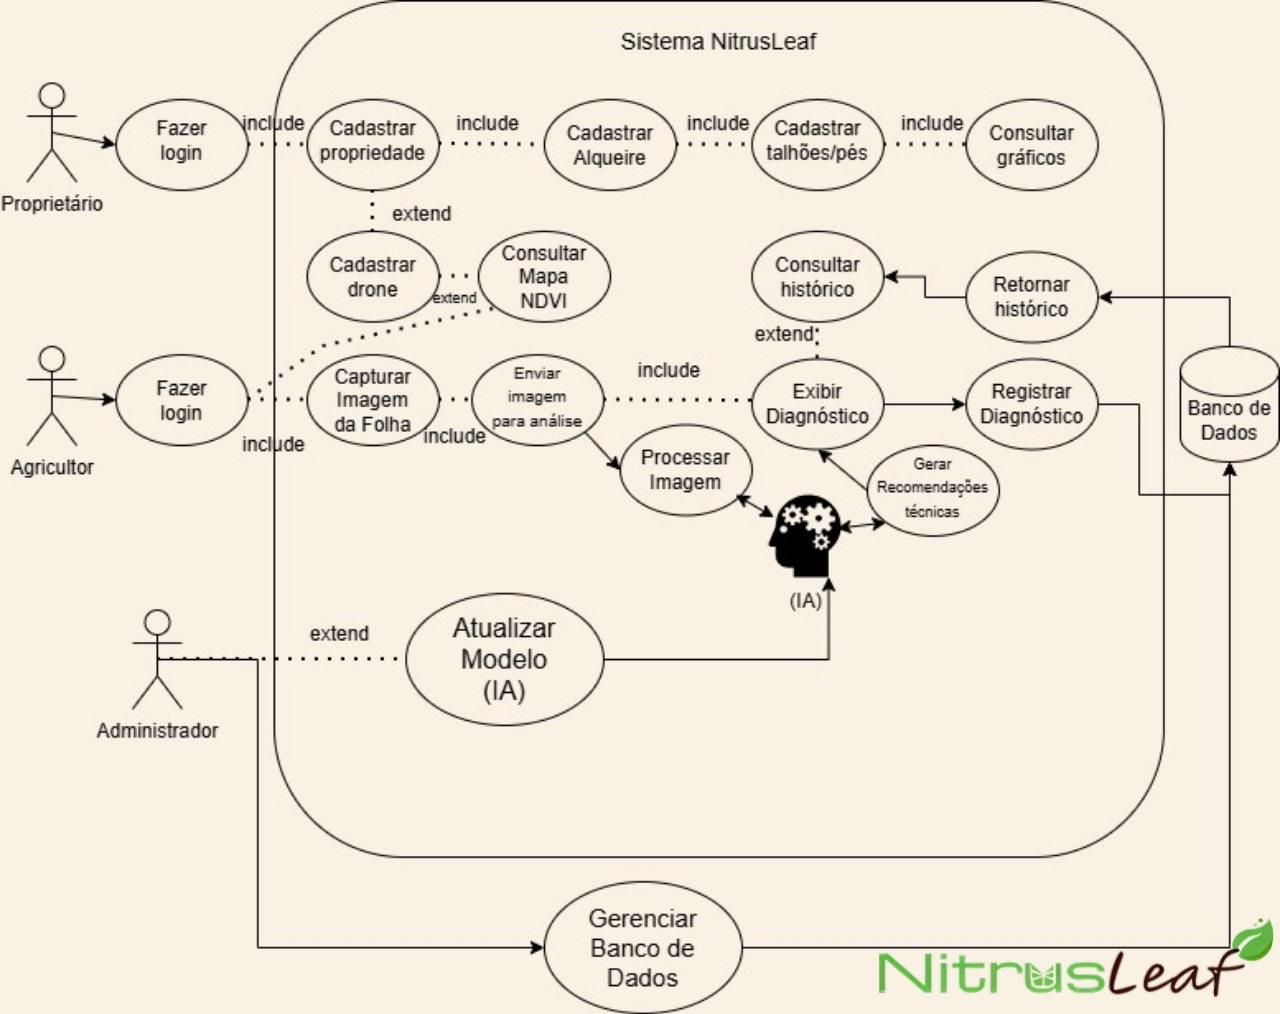
\includegraphics[width=0.8\textwidth]{Images/DiagramaCasosDeUso.jpg}
\SourceOrNote{Equipe 21 - Vitalliz (2025)}
\end{figure}

O diagrama acima ilustra as principais interações entre os usuários e o sistema,
evidenciando os processos relacionados ao monitoramento de deficiências nutricionais
em plantações de mexerica com o apoio de tecnologia de drones.
\medskip

% ------------------------------------------------------------------
    \subsection{\textbf{Diagrama de Classe}}
    \label{sect:Diagrama-de-classe}
    O diagrama da Figura 2 resume um sistema de gestão agrícola com classes para Usuário, Propriedade, Talhão e 
Diagnóstico, além de ServidorNode, ProcessamentoPython, BancoDeDados e PainelAdmin. Juntas, elas cobrem do 
login e cadastro ao registro de áreas, classificação de imagens por CNN e armazenamento/gestão dos resultados.

\medskip
\noindent{As principais classes e seus papéis são:}
\begin{itemize}[itemsep=0.6em, topsep=0.3em, parsep=0pt]
    \item \textbf{Propriedade}: Cadastra e gerencia propriedades rurais (endereço completo, cidade, CEP), vinculadas a um idUsuario; permite criar/editar e listar talhões da propriedade.
    \item \textbf{Usuario}: Mantém dados pessoais e de autenticação (nome, e-mail, telefone, senha, tipo); oferece cadastro, edição de perfil e login para controle de acesso.
    \item \textbf{Talhao}: Subárea da propriedade. Guarda id e nome, ligado a uma Propriedade. Permite cadastrar/editar e consultar o histórico de diagnósticos do local.
    \item \textbf{Diagnostico}: Registro de análise por imagem de folha. Liga-se a um Talhão e salva data, resultado e probabilidade. Métodos: enviar imagem, receber e visualizar resultado.
    \item \textbf{ServidorNode}: Faz a ponte do frontend com a API; recebe requisições, encaminha para o módulo Python, monitora status e salva resultados no banco.
    \item \textbf{ProcessamentoPython}: Executa classificação de imagens com CNN, controla versões dos modelos e permite atualizar/rodar modelos para análise agrícola.
    \item \textbf{BancoDeDados}: Gerencia a conexão e as operações CRUD; insere, consulta e atualiza registros, sustentando a persistência de todo o sistema.
    \item \textbf{PainelAdmin}: Área do administrador para gestão global; visualiza usuários, monitora o sistema e atualiza modelos de CNN, garantindo o controle da plataforma.
\end{itemize}

\begin{figure}[H]
\centering
\caption{Diagrama de classe}%
\label{fig:diagrama-classe}
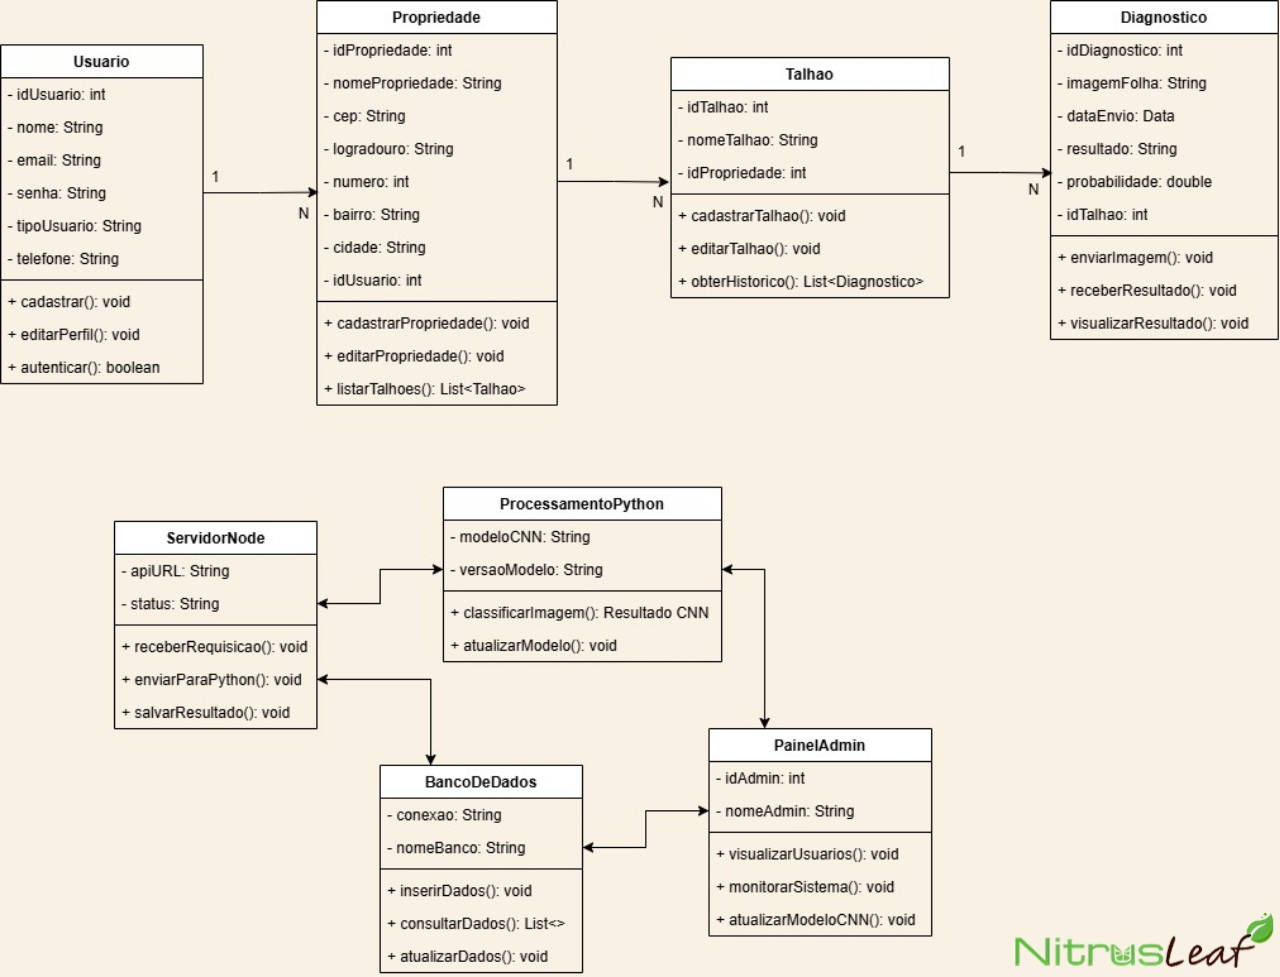
\includegraphics[width=0.8\textwidth]{Images/DiagramaDeClasses.jpg}
\SourceOrNote{Equipe 21 - Vitalliz (2025)}
\end{figure}

O diagrama mostra claramente os relacionamentos de composição e agregação
entre as entidades, com cardinalidades bem definidas. Além disso, os métodos estão
especificados em várias classes, indicando a lógica operacional do sistema, e a
estrutura geral está organizada para refletir um fluxo de uso coerente com os casos de
uso anteriores.
\medskip

% ---------------------------------------------------------- --------
    \subsection{\textbf{Diagrama de Objetos}}
    \label{sect:Diagrama-de-objetos}
    O diagrama de objetos a seguir exemplifica, com instâncias concretas, partes do sistema previamente modelado:
são criados objetos de CadastrarDadosUsuario (abrangendo usuários dos tipos físico e jurídico), 
CadastrarDadosPropriedade e CadastrarTalhão, evidenciando o fluxo de criação e vinculação entre eles. Assim, 
o exemplo mostra como um usuário é instanciado com seus atributos, em seguida uma propriedade é cadastrada e 
associada a esse usuário, e por fim um talhão é criado e ligado à propriedade, ilustrando de forma prática 
as relações e o ciclo de cadastro definidos no diagrama de classes.

\begin{figure}[H]
\centering
\caption{Diagrama de objetos}%
\label{fig:diagrama-objetos}
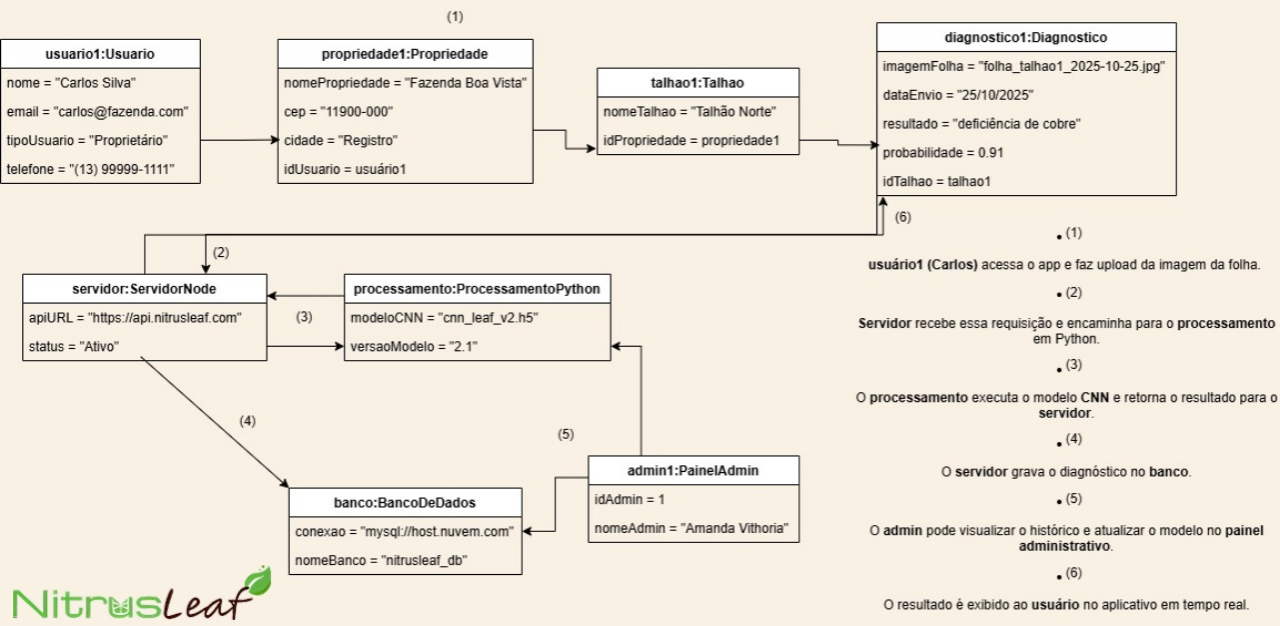
\includegraphics[width=0.8\textwidth]{Images/DiagramaDeObjetos.jpg}
\SourceOrNote{Equipe 21 - Vitalliz (2025)}
\end{figure}

O diagrama usa valores realistas (nomes, CEP, cidade, URLs) e encadeia o fluxo completo
do upload da folha pelo produtor até o diagnóstico gravado e exibido, com supervisão do admin
e versionamento do modelo.
\medskip

% ------------------------------------------------------------------

% --- Diagramas de Banco de Dados ---
\section{Diagramas de Banco de Dados}{Diagramas de Banco de Dados}
A seguir são apresentados os diagramas de banco de dados que ilustram a
estrutura e os relacionamentos das tabelas utilizadas no sistema.

% ------------------------------------------------------------------
    \subsection{\textbf{Diagrama Entidade-Relacionamento (DER)}}
    \label{sect:Diagrama-Entidade-Relacionamento}
    
\medskip
O diagrama a seguir representa o Modelo Entidade–Relacionamento (DER) do sistema \textit{Nitrusleaf}, 
descrevendo a estrutura lógica do banco de dados. As entidades, seus atributos e os relacionamentos 
foram definidos conforme os requisitos do sistema, assegurando integridade e suporte às funcionalidades 
de operação e análise.

\medskip
A entidade \textbf{Usuários} centraliza as informações de acesso e cadastro 
(incluindo \textit{tipo\_pessoa}, foto, CPF/CNPJ e dados de contato/endereço). Ela se relaciona 
com \textbf{Propriedades} pelo relacionamento \textbf{Possui}: um usuário pode não possuir ou 
possuir várias propriedades (0:N) e cada propriedade pertence a um único usuário (1:1).
\medskip

As \textbf{Propriedades} armazenam dados cadastrais (logradouro, CEP, cidade) e contadores globais 
(\textit{talhoes\_registrados}, \textit{total\_pes}). Cada propriedade \textbf{contém} múltiplos 
\textbf{Talhões} (1:N) e também \textbf{contém} diversos \textbf{Alqueires} (1:N). Os \textbf{Talhões} 
registram metadados produtivos (espécie/fruta, \textit{total\_pes}, \textit{pes\_analisados}, 
\textit{pes\_diagnosticados}).
\medskip

Dentro de cada talhão são cadastrados os \textbf{Pés} (plantas individuais), em relacionamento 1:N 
(Talhão~$\rightarrow$~Pés). A entidade \textbf{Pés} guarda a situação atual e campos de diagnóstico 
(\textit{deficiencia\_cobre}, \textit{deficiencia\_manganes}, \textit{outros}, \textit{observacoes}).
\medskip

O histórico temporal de cada planta é mantido por \textbf{Historico\_pe}, ligado a \textbf{Pés} pelo 
relacionamento \textbf{Armazena}: um pé pode possuir muitos registros (descrição, \textit{data\_criacao}, 
situação) e cada registro referencia um único pé (e seu talhão no momento do evento).
\medskip

As avaliações visuais são registradas em \textbf{Fotos}. Pelo relacionamento \textbf{Analisado\_por}, 
um Pé pode ter muitas fotos (1:N) e cada Foto está vinculada a um único pé (URL, \textit{data\_tiragem}, 
\textit{resultado\_analise}).
\medskip

A partir das fotos, o sistema gera \textbf{Relatórios}. Cada Relatório é produzido a partir de uma 
única Foto e vincula-se a um único Pé, consolidando \textit{data da análise}, achados de deficiência 
(cobre, manganês, outros) e observações. O relacionamento \textbf{Tem\_relatorios} expressa que um pé 
pode possuir vários relatórios (1:N), e \textbf{Gera} indica a origem do relatório a partir de uma foto 
(uma foto pode originar relatórios reprocessados).
\medskip

\begin{figure}[H]
\centering
\caption{Diagrama Entidade–Relacionamento}
\label{fig:diagrama-der}
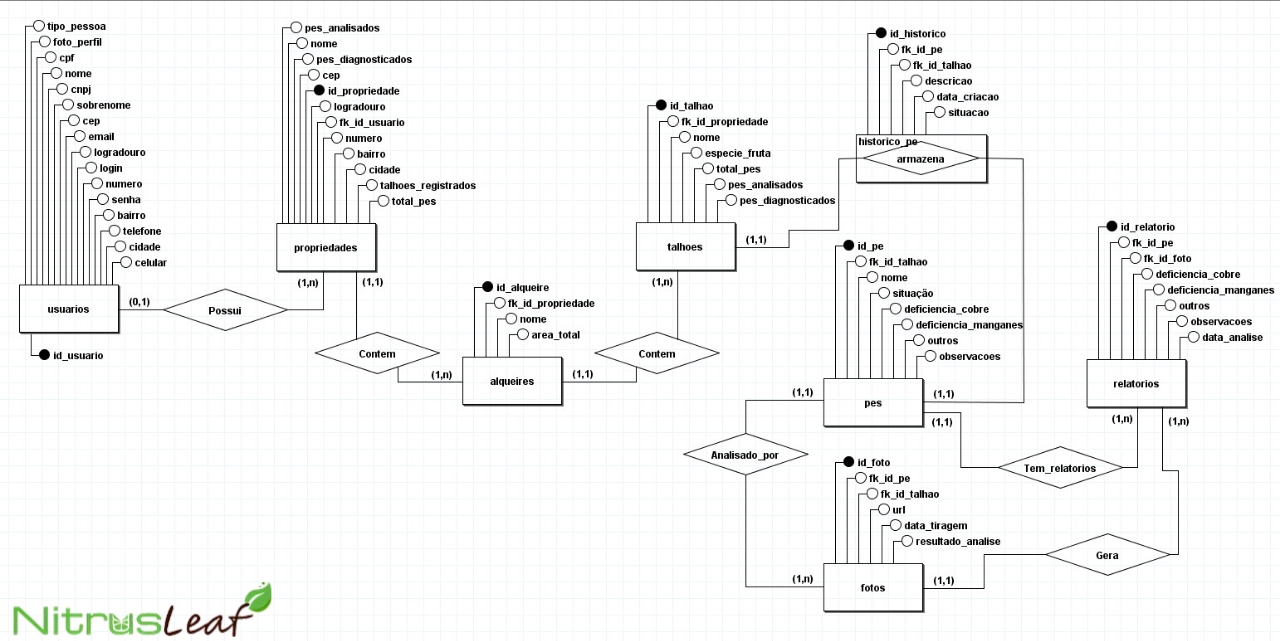
\includegraphics[width=0.9\textwidth]{Images/DiagramaDER.jpg}
\SourceOrNote{Equipe 21 -- Vitalliz (2025)}
\end{figure}

Esse modelo é fundamental para garantir a integridade dos dados e a correta
estruturação das informações no sistema.
\medskip

% ------------------------------------------------------------------
    \subsection{\textbf{Diagrama Modelo Lógico (MER)}}
    \label{sect:Diagrama-Modelo-Lógico}
    \input{Topicos/Diagrama-Modelo-Lógico}


% --- Canvas ---
\section{Modelo de Negócios Canvas}
A seguir são apresentados os diagramas de banco de dados que ilustram a
estrutura e os relacionamentos das tabelas utilizadas no sistema.

\label{sect:Canvas}
\medskip
\noindent\textbf{Proposta de Valor}\\
O sistema tem como objetivo central ajudar os agricultores a identificarem deficiências de manganês e cobre nas folhas de mexerica, contribuindo para manter o padrão de qualidade da fruta. A utilização de inteligência artificial integrada ao sistema oferece precisão na análise das fotos enviadas pelos usuários.

\medskip
\noindent\textbf{Segmento de Mercado}\\
O público-alvo são os agricultores de mexerica do Vale do Ribeira, com foco específico em produtores rurais, horticultores e demais interessados na melhoria da produtividade agrícola.

\medskip
\noindent\textbf{Relacionamento com o Cliente}\\
O relacionamento com os usuários será realizado via WhatsApp, aplicativo móvel e site institucional. Os usuários poderão enviar fotos das folhas e receber feedback automatizado por meio de gráficos e mapas gerados pelo sistema. O aplicativo também permite o envio de análises e resultados personalizados.

\medskip
\noindent\textbf{Canais}\\
A divulgação e o acesso ao sistema ocorrerão por meio de anúncios em secretarias de agricultura dos municípios da região, com suporte adicional via site, e-mail e WhatsApp da empresa, fortalecendo a comunicação direta com o público-alvo.

\medskip
\noindent\textbf{Atividades-Chave}\\
As principais atividades envolvem a identificação de deficiência nutricional nas folhas e o fornecimento de suporte técnico e manutenção contínua do sistema.

\medskip
\noindent\textbf{Recursos-Chave}\\
Para operar corretamente, o sistema depende de uma equipe técnica composta por programadores, instaladores do sistema físico e profissionais responsáveis pelo suporte online. Além disso, é necessário um serviço de hospedagem para o site e para o banco de dados.

\medskip
\noindent\textbf{Parcerias-Chave}\\
As parcerias incluem associações de fazendeiros, secretarias de agricultura locais e participação em feiras do setor agrícola, que auxiliam na disseminação e na credibilidade do projeto.

\medskip
\noindent\textbf{Estrutura de Custos}\\
Inclui gastos com manutenção dos equipamentos de monitoramento, aluguel de espaço físico para atendimento, aquisição de materiais e tecnologias para análise das folhas, além de custos com servidores para armazenamento dos dados.

\medskip
\noindent\textbf{Fontes de Renda}\\
A monetização ocorre por meio do aluguel do sistema, da cobrança pelo aluguel de equipamentos necessários e da prestação de serviços de instalação e manutenção.
\medskip

\begin{figure}[H]
\centering
\caption{Modelo de Negócios Canvas}
\label{fig:Canvas}
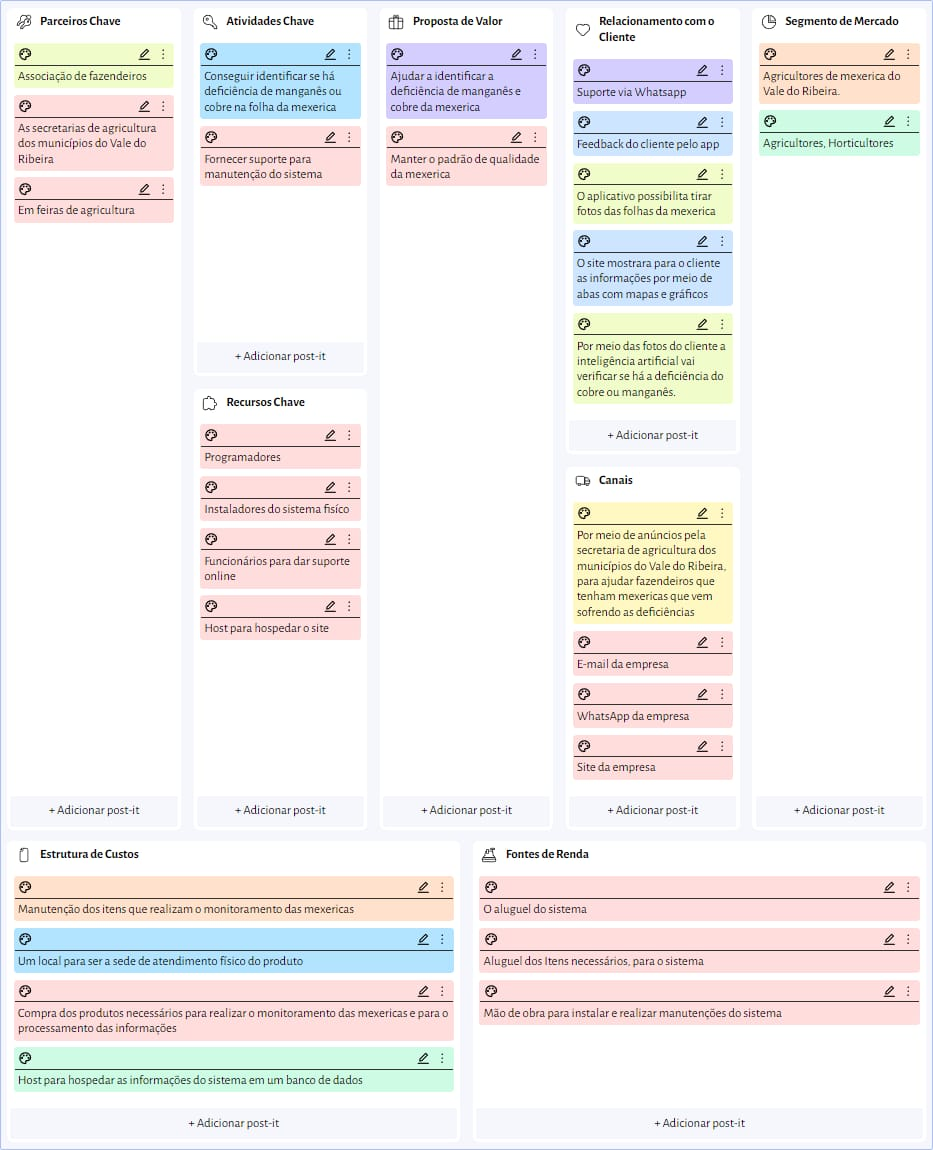
\includegraphics[width=0.8\textwidth]{Images/Canvas.jpeg}
\SourceOrNote{Equipe 21 - Vitalliz (2025)}
\end{figure}
\medskip


% --- Diagramas de Redes ---
\section{DIAGRAMA E ESPECIFICAÇÕES DA INFRAESTRUTURA DE REDE}
Esta seção descreve a estrutura lógica e física da rede interna utilizada para o
funcionamento do sistema de monitoramento e análise de folhas de mexerica,
conforme representado no diagrama a seguir.

% ------------------------------------------------------------------
    \subsection{\textbf{Visão Geral da Rede}}
    \label{sect:Visao-geral-da-Rede}
    

A infraestrutura NitrusLeaf centraliza o diagnóstico agrícola, onde o Agricultor envia imagens de 
plantas via internet (HTTPS) para o Servidor da Sede, que as processa usando Inteligência Artificial 
(IA) para identificar problemas. Os resultados são armazenados em um Banco de Dados na Nuvem e 
o servidor devolve ao usuário um diagnóstico e uma recomendação prática. O sistema é mantido e aprimorado
por um Administrador que atualiza os modelos de IA, garantindo a segurança dos dados e a precisão das 
análises de campo

% ------------------------------------------------------------------
    \subsection{\textbf{Componentes da Rede}}
    \label{sect:Componentes-da-Rede}
    \noindent\textbf{Nuvem (Servidor Externo:)}\par
Hospeda os serviços centrais do sistema: \textit{API Node.js} (ponto de entrada das requisições), 
\textit{Banco MySQL} (armazenamento de propriedades, diagnósticos, imagens e histórico) e 
\textit{Processamento de Imagens (IA)} (análises e geração de resultados). A comunicação externa 
ocorre via \textbf{HTTPS/TLS}, enquanto a comunicação interna entre serviços permanece em sub-redes 
privadas com regras de segurança (grupos de segurança/firewall). Proporciona \textit{escala}, 
\textit{alta disponibilidade} e \textit{monitoramento/logs} para auditoria e desempenho.

\medskip
\noindent\textbf{Roteador (Acesso do Cliente:)}\par
Responsável por interligar a \textbf{rede local da propriedade} à internet (fibra/rádio/4G--5G). 
Encaminha o tráfego \textbf{HTTPS} dos dispositivos dos usuários até a API na nuvem e recebe as respostas
(diagnóstico e recomendações). Executa \textit{NAT}, pode fornecer \textit{DHCP} e aplicar \textit{QoS} 
para priorizar upload de imagens. Opcionalmente estabelece \textit{VPN} para gestão remota segura e 
implementa políticas básicas de firewall na borda do cliente.

\medskip
\noindent\textbf{Rede (LAN \& WAN:)}\par
A \textbf{LAN da Propriedade} conecta os endpoints (PC do Proprietário e smartphone do Agricultor) 
por cabo/wi-fi, podendo usar \textit{switch} para segmentação e ampliação de portas. A 
\textbf{WAN (Internet/Nuvem)} é o meio público IP que transporta os dados entre cliente e serviços 
em nuvem com \textbf{TLS} de ponta a ponta. Fluxo típico: \textit{Dispositivo} $\rightarrow$ 
\textit{Roteador (LAN)} $\rightarrow$ \textit{Internet (WAN)} $\rightarrow$ 
\textit{API Node.js (Nuvem)} $\rightarrow$ \textit{MySQL/IA (Nuvem)} $\rightarrow$ 
\textit{Resposta ao usuário}.
\medskip

% ------------------------------------------------------------------
    \subsection{\textbf{Fluxo de Comunicação}}
    \label{sect:Fluxo-de-comunicacao}
    \noindent\textbf{Internamente (Rede)}
\begin{itemize}
    \setlength{\itemsep}{0.8em}   % espaço entre itens
    \setlength{\topsep}{0.4em}    % espaço antes/depois da lista
    \setlength{\parsep}{0pt}      % espaço entre parágrafos dentro do item
    \setlength{\parskip}{0pt}
    \item \textbf{Switch}: interliga os computadores dos setores (desenvolvimento, manutenção e recepção) na LAN, comutando o tráfego local.
    \item \textbf{Roteador (NAT/Firewall)}: conecta a LAN à Internet, aplica NAT e regras de firewall, garantindo que os hosts internos acessem serviços externos com segurança.
    \item \textbf{Saída para a Internet}: provê conectividade externa para o acesso ao site/app e para a comunicação com a API.
\end{itemize}

\medskip
\noindent\textbf{Externamente (Cliente \(\leftrightarrow\) Sede via Internet)}
\begin{itemize}
    \setlength{\itemsep}{0.8em}
    \setlength{\topsep}{0.4em}
    \setlength{\parsep}{0pt}
    \setlength{\parskip}{0pt}
    \item \textbf{Canal}: comunicação realizada via \textbf{HTTPS} sobre a Internet pública.
    \item \textbf{Fluxo de alto nível}: o cliente envia imagens \(\rightarrow\) o tráfego chega à \textbf{API (Servidor Node.js)} \(\rightarrow\) a API orquestra processamento/armazenamento \(\rightarrow\) o diagnóstico é retornado ao cliente (site/app).
    \item \textbf{Observações de rede}: o cliente \textbf{não acessa diretamente} o módulo de IA nem o banco; a LAN permanece isolada atrás do NAT do roteador.
\end{itemize}
\medskip

% ------------------------------------------------------------------
    \subsection{\textbf{Segurança e Estabilidade}}
    \label{sect:Seguranca-e-estabilidade}
    \medskip
\noindent{Para garantir a estabilidade da comunicação e a segurança dos dados:}
\begin{itemize}
    \item Utiliza-se autenticação segura no acesso ao sistema;.
    \item O tráfego de informações entre o usuário e o servidor é criptografado;
    \item O roteador é configurado com firewall e controle de acesso;
    \item O servidor é mantido em ambiente cloud com redundância e backups regulares.
\end{itemize}

\medskip

\begin{figure}[H]
\centering
\caption{Diagrama Infraestrutura de Redes}
\label{fig:diagrama-infraestrutura}
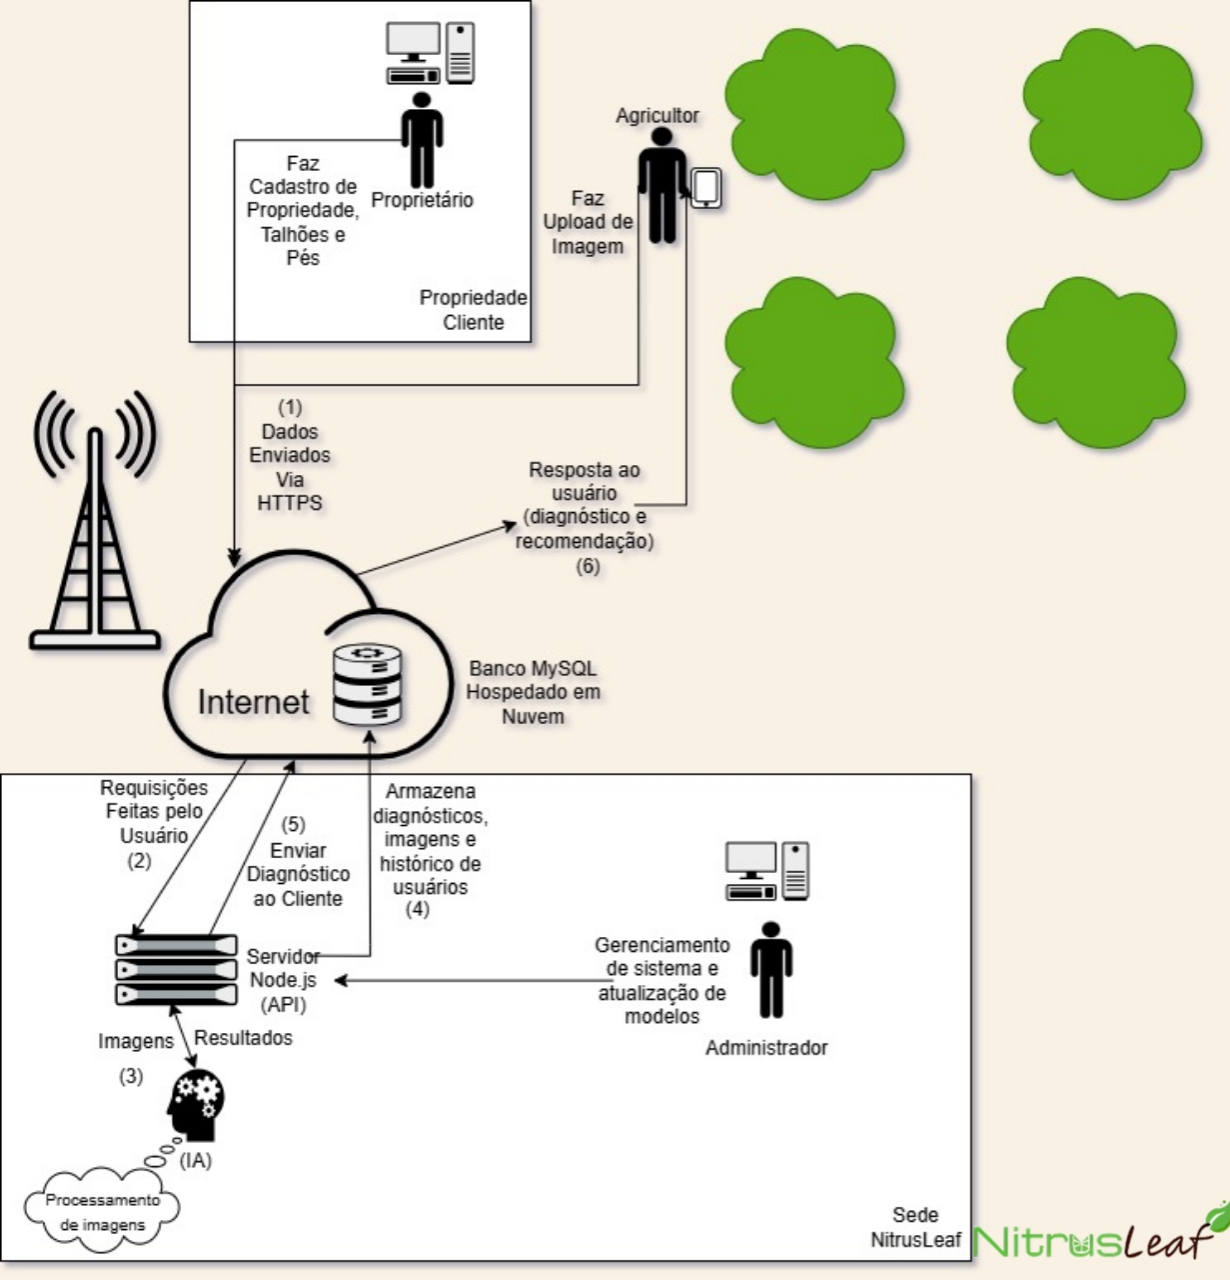
\includegraphics[width=0.8\textwidth]{Images/DiagramaInfraestruturaDeRedes.jpg}
\SourceOrNote{Equipe 21 - Vitalliz (2025)}
\end{figure}
\medskip

A infraestrutura de rede integra clientes à Nuvem via HTTPS para processamento por 
IA e persistência de dados no MySQL, sendo orquestrada por uma API Node.js, o que garante segurança, 
escalabilidade e gestão centralizada.
\medskip

% --- UI de Alta Fidelidade (Figma) ---
\section{Interface de Usuário de Alta Fidelidade (Figma)}
\medskip
Esta seção apresenta as principais telas do sistema desenvolvidas para os usuários
finais. O sistema foi projetado no Figma com foco na usabilidade, acessibilidade e praticidade no
monitoramento e análise de deficiências nutricionais nas folhas de mexerica.


\clearpage
\end{document}